\documentclass{article}
\usepackage{graphicx} % Required for inserting images
\usepackage{tabularx}
\usepackage{float}
\usepackage{longtable}
\usepackage[export]{adjustbox}

\title{Obliczenia Naukowe Lista 4}
\author{Bartłomiej Puchała}
\date{December 2023}

\begin{document}

\maketitle

\section{Zadanie 1}
\subsection{Opis problemu}
Problem polega na napisaniu funkcji obliczającej ilorazy różnicowe. Ilorazy różnicowe są wykorzystywane do budowy wielomianu interpolacyjnego. Funkcję należy zaprogramować bez użycia tablicy dwuwymiarowej mając podane jako parametry:
\begin{center}

\begin{enumerate}
    \item x - wektor długości $n + 1$ zawierający węzły $x_0$,...$x_n$ gdzie $x[1] = x_0$,...,$x[n+1] = x_n$
    \item f - wektor długości $n + 1$ zawierający wartości interpolowanej funkcji w węzłach $f(x_0)$,...,$f(x_n)$
\end{enumerate}

\end{center}
\subsection{Rozwiazanie}
Rozwiazanie polega na obliczeniu ilorazów różnicowych za pomocą podanej reukrencji:
$$f[x_0] = f(x_0)$$
$$f[x_i, x_j] = \frac{f[x_j] - f[x_i]}{x_j - x_i}$$
$$ f[x_0, x_1, ..., x_n] = \frac{f[x_1, x_2, ..., x_n] - f[x_0, x_1, ..., x_{n-1}]}{x_n - x_0} $$
Aby nie wykorzystywać tablicy dwuwymiarowej należy wypełnić tablicę na początku wartościami węzłów $x_i$ funkcji $f$, a potem przy kolejnej iteracji rzędu aktualizować obliczone ilorazy przeliczając je kolejny raz od dołu. W ten sposób zostaną uwzględnione wcześniej wyliczone ilorazy różnicowe, od których sa zależne.
\newpage
Ta funkcja znajduje się w module Functions.jl
\vspace{10pt}
\begin{verbatim}
function ilorazyRoznicowe(x::Vector{Float64}, f::Vector{Float64})
    n = length(f)
    # fx[1] = f[1] # c0 = f(x0)
    # Algorytm Newtona wzoru interpolacyjnego

    res = [value for value in f]
    println(res)
    println("-----")
    for i in 1:n
        for j in n:-1:i+1
            res[j] = (res[j] - res[j-1]) / (x[j] - x[j - i])
        end
    end
    return res
end
\end{verbatim}
\section{Zadanie 2}
\subsection{Opis problemu}
Problem polega na napisaniu funkcji obliczającej wartość wielomianu interpolacyjnego stopnia $n$ w postaci Newtona $N_n(x)$ w punkcie $x = t$ za pomocą uogólnionego algorytmu Hornera w czasie $O(n)$. Parametrami funkcji są:
\begin{center}
$x$ - wektor długości $n + 1$ zawierający węzły $x_0$, ..., $x_n$, gdzie $x[1] = x_0$, ..., $x[n+1] = x_n$
\vspace{5pt}

$fx$ - wektor długości $n + 1$ zawierający ilorazy różnicowe, gdzie $fx[1] = f[x_0]$, $fx[2] = f[x_0, x_1]$, ..., $fx[n] = f[x_0, ..., x_{n-1}]$, $fx[n+1] = f[x_0, ..., x_n]$
\vspace{5pt}

$t$ - punkt, w którym należy obliczyć wartość wielomianu
\end{center}
\subsection{Rozwiazanie}
Algorytm korzysta z uogólnionego algorytmu Hornera, który przedstawia się następująco:
$$ w_n(x) := f[x_0, x_1, ..., x_n] $$
$$ w_k(x) := f[x_0, x_1, ..., x_k] + (x - x_k)w_{k + 1}(x) (k = n - 1, ..., 0)$$
$$ N_n(x) := w_0(x) $$

$f[x_0, x_1, ..., x_n]$ jest ilorazem różnicowym stopnia $n$ dla funkcji $f(x)$ względem węzłów $x_0, x_1, ..., x_n $. Oznacza on tempo zmiany funkcji w danym punkcie interpolacyjnym.
\begin{verbatim}
Ta funkcja znajduje się w module Functions.jl
function warNewton(x::Vector{Float64}, fx::Vector{Float64}, t::Float64)
    n = length(fx)
    nt = fx[n] # wn(x) = f[x0, ..., xn] warunek poczatkowy
    for k in n-1:-1:1
        nt = fx[k] + (t - x[k]) * nt
    end
    return nt
end
\end{verbatim}

\section{Zadanie 3}
\subsection{Opis problemu}
Problem polega na napisaniu funkcji obliczającej w czasie $O(n^2)$ współczynniki postaci naturalnej wielomianu $a_0, ..., a_n$ tzn. $a_nx^n + a_{n-1}x^{n-1} + ... + a_1x + a_0$ znając współczynniki wielomianu interpolacyjnego w postaci Newtona $c_0 = f[x_0]$, $c_1 = f[x_0, x_1] $ oraz węzły $x_0, x_1, ..., x_n$.
\subsection{Rozwiazanie}
Wielomian w postaci interpolacyjnej przedstawia się następująco: 
$$ N_n(x) = f[x_0] + f[x_0, x_1](x - x_0) + f[x_0, x_1, x_2](x - x_0)(x - x_1) + ... + f[x_0, x_1, ..., x_n](x - x_0)(x-x_1)...(x-x_{n-1})$$
Współczynnikiem $a_n$ stojącym przy najwyższej potędze $x^n$ jest $c_n$. Startując od najwyższych potęg można przy kolejnych przejściach aktualizować współczynniki przy odejmowanych aktualnie potęgach w ten sposób, że są one w postaci naturalnej. Przy iteracjach wykorzystane zostaną obliczone wcześniej współczynniki częściowe postaci naturalnej do zaktualizowania ich o nowe potęgi.
\begin{verbatim}
Ta funkcja znajduje się w module Functions.jl
function naturalna(x::Vector{Float64}, fx::Vector{Float64})
    n = length(fx)
    a = [val of val in fx]

    for i in n-1:-1:1
        a[i] = fx[i] - a[i + 1] * x[i]
        for j in i+1:n-1
            a[j] = a[j] - a[j + 1] * x[i]
        end
    end

    return a
end
\end{verbatim}

\section{Zadanie 4}
\subsection{Opis problemu}
Zadanie polega na napisaniu funkcji, która zinterpoluje zadaną funkcję $f(x)$ w przedziale $[a,b]$ za pomocą wielomianu interpolacyjnego stopnia $n$ w postaci Newtona. Należy narysować wielomian interpolacyjny i interpolowaną funkcję.
\subsection{Rozwiazanie}
Ta funkcja znajduje się w module Functions.jl
\begin{verbatim}
function rysujNnfx(f, a::Float64, b::Float64, n::Int)
    if a > b
        a, b = b, a
    end

    x = Vector{Float64}(undef, n + 1)
    y = Vector{Float64}(undef, n + 1)
    delta = zero(Float64)

    for k in 1:n+1
        x[k] = a + delta
        y[k] = f(x[k])
        delta += (b - a) / n
    end


    ilorazy = ilorazyRoznicowe(x, y)
    interpolationX = Vector{Float64}(undef, n + 1)
    interpolationY = Vector{Float64}(undef, n + 1)
    realVals = Vector{Float64}(undef, n + 1)

    delta = zero(Float64)
    for i in 1:n+1
        interpolationX[i] = a + delta
        interpolationY[i] = warNewton(x, ilorazy, interpolationX[i])
        realVals[i] = f(interpolationX[i])
        delta += (b - a) / n
    end

    clf()
    plot(interpolationX, interpolationY, label = "interpolated", linewidth = 1.5)
    plot(interpolationX, realVals, label = "f(x)", linewidth = 1.5, alpha = 0.5)
    legend(title = "Interpolacja")
    savefig(string("wykresy/plot", f, "-", n, ".png"))
end
\end{verbatim}

\section{Zadanie 5}
\subsection{Opis problemu}
Problem polega na przetestowaniu funkcji rysujNnfx(f, a, b, n) na przykładach:
\begin{enumerate}
    \item $e^x$, $[0,1]$, $n = 5,10,15,$
    \item $x^2sin(x)$, $[-1,1]$, $n = 5,10,15,$
\end{enumerate}
\subsection{Rozwiazanie}
\begin{figure}[H] 
\centering
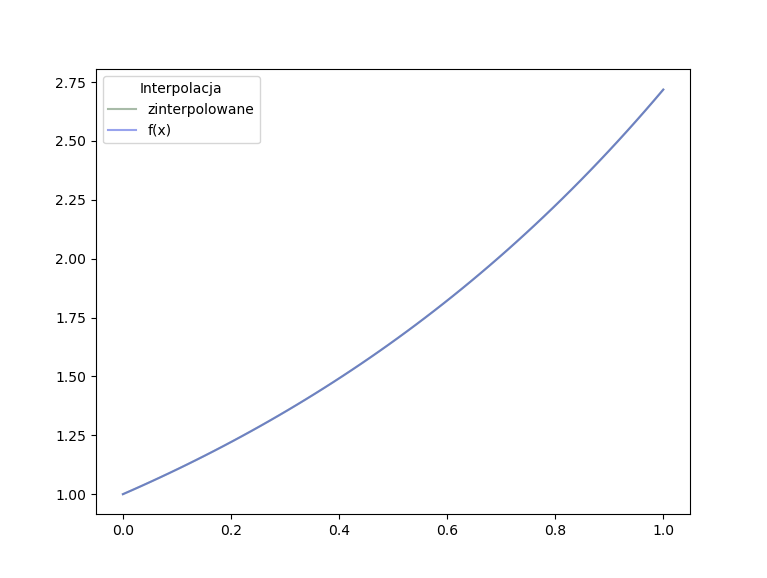
\includegraphics[width=0.85\textwidth, height=6.5cm]{e_x_5.png}
\caption{e^x, n = 5}
\label{e_x_5}
\end{figure}

\begin{figure}[H] 
\centering
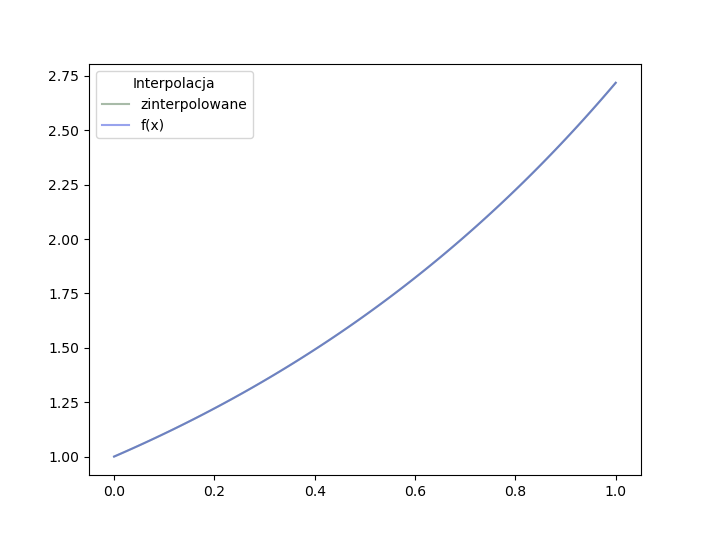
\includegraphics[width=0.85\textwidth, height=6.5cm]{e_x_10.png}
\caption{e^x, n = 10}
\label{e_x_10}
\end{figure}

\begin{figure}[H] 
\centering
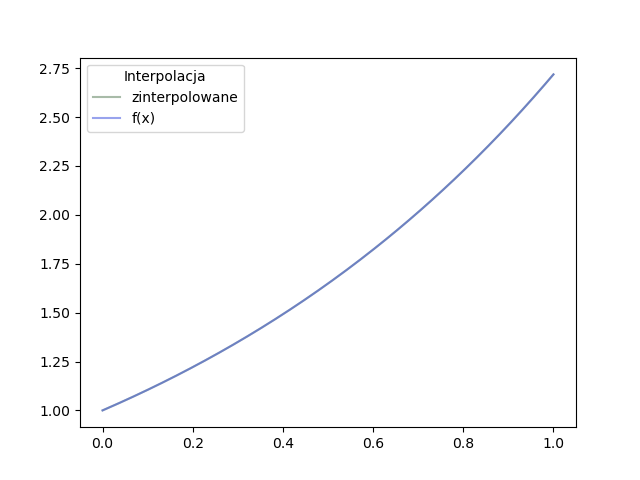
\includegraphics[width=0.85\textwidth, height=6.5cm]{e_x_15.png}
\caption{e^x, n = 15}
\label{e_x_15}
\end{figure}

\begin{figure}[H] 
\centering
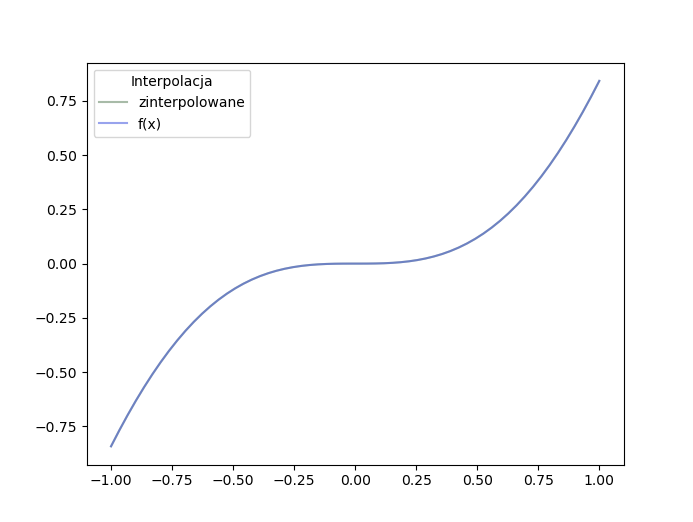
\includegraphics[width=0.8\textwidth, height=6.5cm]{sin_5.png}
\caption{x^2sin(x), n = 5}
\label{x^2sin(x)_5}
\end{figure}

\begin{figure}[H] 
\centering
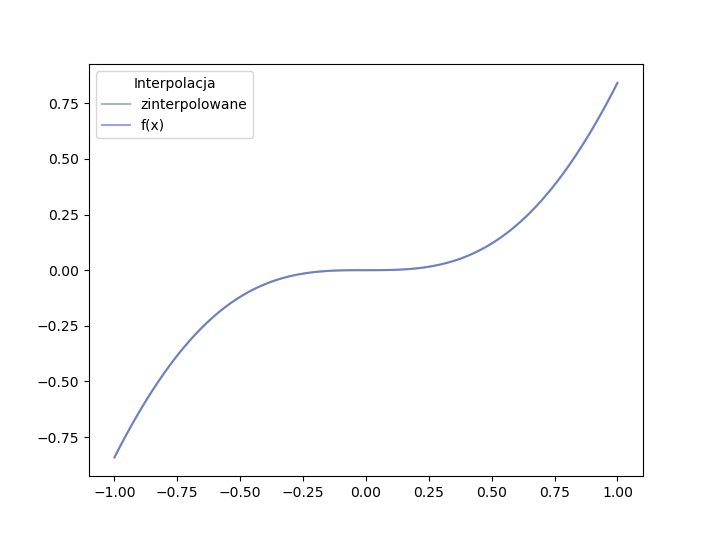
\includegraphics[width=0.8\textwidth, height=6.5cm]{sin_10.png}
\caption{x^2sin(x), n = 10}
\label{x^2sin(x)_10}
\end{figure}

\begin{figure}[H] 
\centering
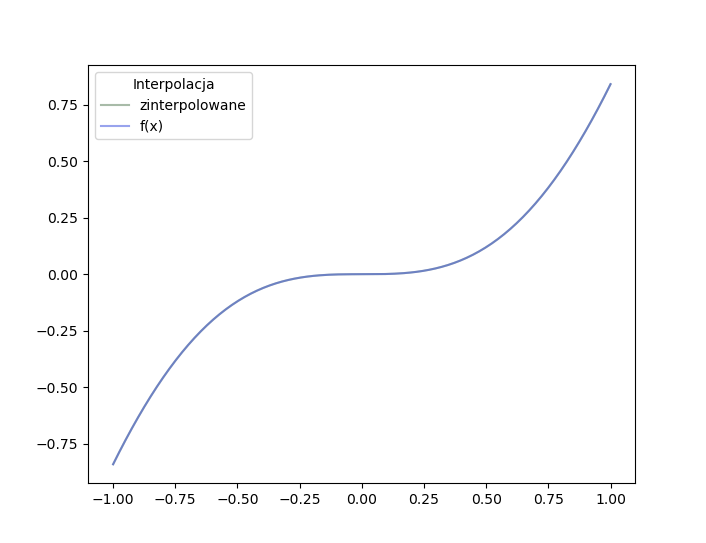
\includegraphics[width=0.85\textwidth, height=6.5cm]{sin_15.png}
\caption{x^2sin(x), n = 15}
\label{x^2sin(x)_15}
\end{figure}

\subsection{Wnioski}
Dla wielomianu interpolacyjnego o małym stopniu wykresy pokrywają się dokładnie. Interpolacja funkcji których zmiana wartości jest niewielka, a pochodna nie zmienia znaku prowadzi do dokładnych wielomianów interpolacyjnych.

\section{Zadanie 6}
\subsection{Opis problemu}
Zadanie polega na pzetestowaniu funkcji z zadania 4 na kolejnych przykładach.
\subsection{Rozwiazanie}

\begin{figure}[H] 
\centering
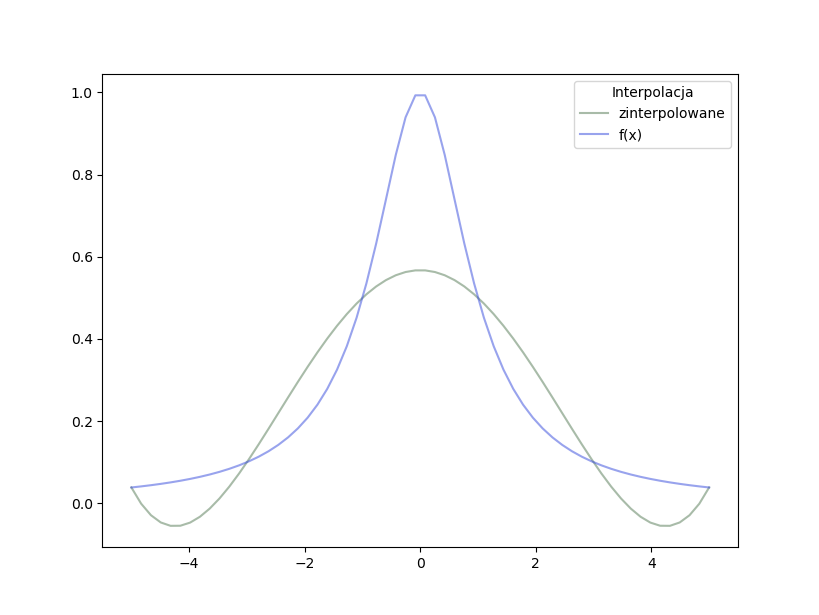
\includegraphics[width=0.85\textwidth, height=6.5cm]{6b_5.png}
\caption{$1 / (1+x^2)$, $n = 5$}
\label{1_(1+x^2)_5}
\end{figure}

\begin{figure}[H] 
\centering
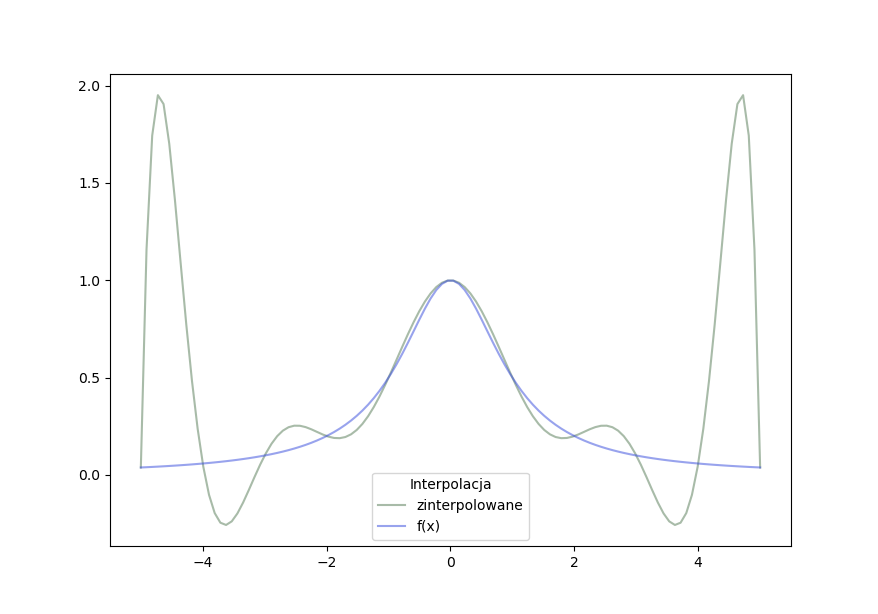
\includegraphics[width=0.85\textwidth, height=6.5cm]{6b_10.png}
\caption{$1 / (1+x^2)$, $n = 10$}
\label{1_(1+x^2)_10}
\end{figure}

\begin{figure}[H] 
\centering
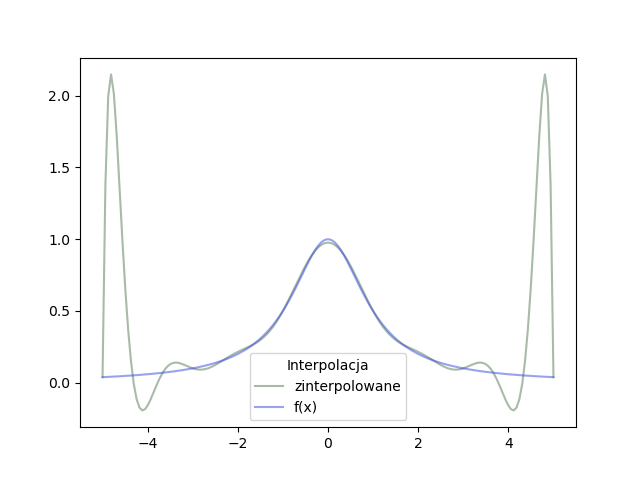
\includegraphics[width=0.85\textwidth, height=6.5cm]{6b_15.png}
\caption{$1 / (1+x^2)$, $n = 15$}
\label{1_(1+x^2)_15}
\end{figure}

\begin{figure}[H] 
\centering
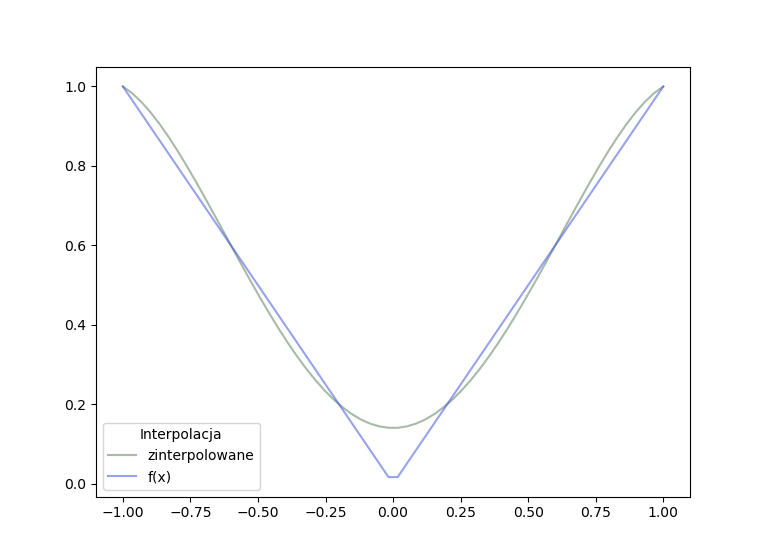
\includegraphics[width=0.85\textwidth, height=6.5cm]{6a_5.png}
\caption{$abs(x)$, $n = 5$}
\label{abs(x)_5}
\end{figure}

\begin{figure}[H] 
\centering
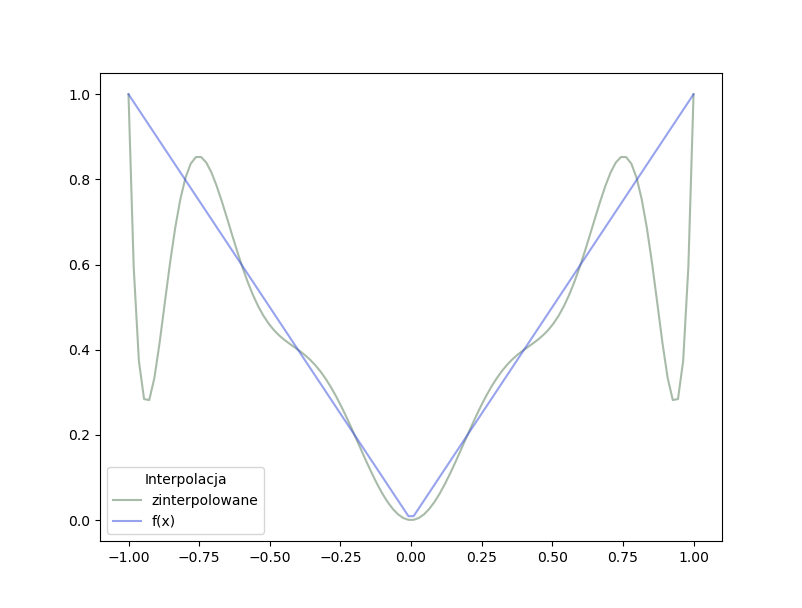
\includegraphics[width=0.85\textwidth, height=6.5cm]{6a_10.png}
\caption{$abs(x)$, $n = 10$}
\label{abs(x)_10}
\end{figure}

\begin{figure}[H] 
\centering
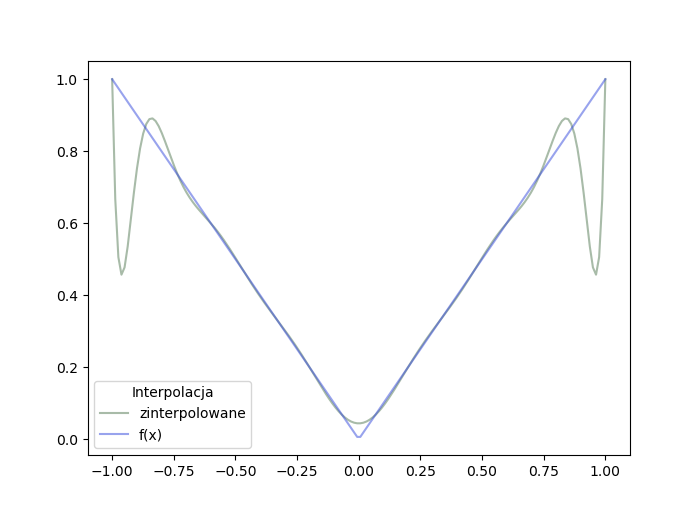
\includegraphics[width=0.85\textwidth, height=6.5cm]{6a_15.png}
\caption{$abs(x)$, $n = 10$}
\label{abs(x)_15}
\end{figure}

\end{document}
